\chapter{Experiment}
\label{cha:experiment}
This chapter describes and analyses an experiment measuring the performance of the previously described authentication mechanisms.
Even if the performance is not the central decision point to choose the correct authentication mechanism, it is still worth considering.
Especially because the migration from a monolithic architecture to the microservice architecture can result in a massive performance decrease of around 79.1\%~\cite{ueda2016workload}.
Therefore the performance is already restricted, and the authentication mechanisms should not produce too much overhead.

\section{Setup}
The setup consists of two components, the service that responds to requests and the client, which performs requests and measures the time taken.
Both components are located in the same network and run on the same machine.
The service is developed in C\# using ASP.Net Core, same as the services of the flea market app, mentioned in chapter~\ref{cha:project_structure}.
The client is a console application developed in C\# using .NET.
The console application is not a microservice, but it acts as a service located within the deployment.
It is not good-practice to access the services directly from an external application bypassing the API Gateway.
Nevertheless, this makes the experiment setup simpler and reduces falsifications by other components. 

The experiment simulates that the client service (the console application) performs 1000 requests to another service.
When the first request is performed, the connection between the services has to be established.
Therefore the first request will take significantly longer since the full TCP handshake and TLS handshake have to be performed.
Following requests can reuse the already created connection and do not have to perform the whole initialization process again.

This experiment does not aim to approximate the expected request durations with the declared technology stack.
Instead, it will compare the trends between the authentication mechanisms.
The exact durations are not relevant since they are influenced by many factors, like the hardware.
The tests were performed five times to minimize distortions between the test runs.

Two different implementations of the approach using self-signed JWTs are compared to the performance using mTLS.
First, an implementation of the self-signed JWT approach, in which a new JWT is created for each request, is shown.
The second implementation uses the same JWT for all requests.
% Unclear antecedent
This should illustrate how the performance using self-signed JWTs can be improved by efficiently reusing the tokens.
Furthermore, the experiment includes the request duration when only TLS is used.
% Unclear antecedent
This should show how much time is accounted by the service-to-service authentication mechanisms and how much time is accounted by other tasks like the transport, the random number generation and the standard TLS-handshake.

\section{Results}

\begin{table}[H]
	\centering
\begin{tabular}{c|c|cc}
	\multicolumn{1}{l|}{\textbf{Authentication Mechanism}} & \textbf{Identifier} & \multicolumn{2}{c}{\textbf{Average Request Duration}} \\ \hline
	\multicolumn{1}{c|}{} & & \multicolumn{1}{c|}{first connection} & reuse connection \\ \hline
	mTLS & $\alpha$ & \multicolumn{1}{c|}{$228.03$ ms} & $9.87$ ms \\ \hline
	self-signed JWT & $\beta$ & \multicolumn{1}{c|}{$193.52$ ms} & $13.57$ ms \\ \hline
	self-signed JWT (reusing token) & $\gamma$ & \multicolumn{1}{c|}{$184.88$ ms} & $8.10$ ms \\ \hline 
	only TLS & $\delta$ & \multicolumn{1}{c|}{$175.78$ ms} & $1.31$ ms
\end{tabular}
\caption{Average request durations of the authentication mechanisms, when random numbers are fetched}
\label{tab:experiment_case_1}
\end{table}

The results of the experiment are shown in table~\ref{tab:experiment_case_1}.
Furthermore, the trend of the average request duration is visualized in figure~\ref{fig:trend}.
% Dangling modifier
To simplify the interpretation of the results, the approaches are identified using the identifiers declared in table~\ref{tab:experiment_case_1}.

According to the experiment results, $\delta$ is the most efficient approach since it only authenticates the server to the client but not the client to the server.
The first request takes only 175.78 ms on average, and the following requests take only 1.31 ms.
Comparing $\delta$ with $\alpha$ shows that $\alpha$ takes in average 8.56 ms longer than $\delta$.
Since the authentication is performed only once per request, it is not valid to say that the request duration between $\delta$ and $\alpha$ increases by 750\%.
The percentual value is only such significant because generating a random number is very simple.
Therefore only the time offsets of this comparison are valuable.
They show that $\alpha$ increases the request duration by 8.56 ms on average compared to $\delta$.
The approaches using self-signed JWTs increase the average request duration by 6.79 ms ($\gamma$) to 12.26 ms ($\beta$) on average compared to $\delta$. 

When mutual authentication is provided, the lowest duration to establish the first connection is achieved using $\gamma$.
% Unclear antecedent
This is reasonable since $\alpha$ has to perform the extended TLS handshake to transfer the certificate and prove that it owns the corresponding private key.
When self signed-JWTs are used, the services have to prove that they own the private key of the transferred certificate by signing the JWTs.
Therefore the extended handshake is unnecessary for the approaches $\beta$ and $\gamma$.
The results show that $\alpha$ takes on average 52.52 ms longer than $\gamma$ to establish the first connection with a service.
$\gamma$ has a minimal advantage of 8.64 ms on average for establishing the first connection compared to $\beta$ because it can reuse a previously generated JWT.

Considering the requests after the connection was established, $\gamma$ is the most efficient approach that provides mutual authentication.
Each request takes about 8.10 ms on average, 1.23 ms less than $\alpha$ and 5.47 ms less than $\beta$.
Nevertheless, it is not possible to reuse the same token for each request in a more realistic example.
Therefore using self-signed JWTs would result in a request duration between $\beta$ and $\gamma$, which is about the request duration of $\alpha$.

\begin{figure}
	\centering
	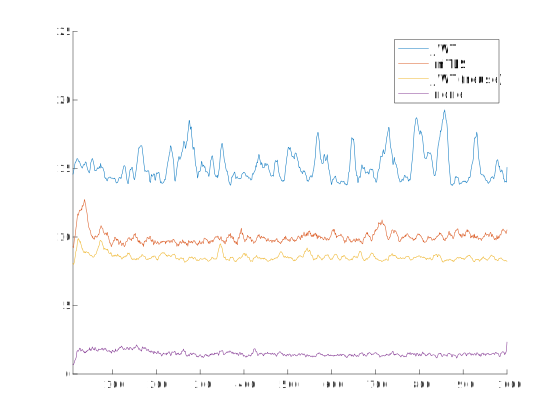
\includegraphics[trim=0 200 0 200, clip, width=\textwidth]{images/experiment/experiment-trend.pdf}
	\caption{Smoothened trend of the average request duration comparing the discussed authentication mechanisms excluding the first request}
	\label{fig:trend}
\end{figure}

\section{Conclusion}
This experiment compared the request durations of the two previous authentication mechanisms.
The results showed that the request durations of the mechanism using self-signed JWTs and mTLS are very similar.
Depending on the implementation of the JWT approach, it can consume up to 34\% more time or up to 20\% less time.
Therefore, performance is not the most crucial criterion when the two authentication mechanisms are compared, because they result in almost similar request durations.

Nevertheless, for time-critical projects in which each millisecond matters, self-signed JWTs are the better choice since the performance can be optimized in multiple ways.
For example, the certificates of the services can be distributed even before the first request is performed.
Or the validity timespan of the tokens can be increased so the same tokens can be used for a longer timespan.
